%!TEX root = ../../main.tex

\begin{frame}[plain]
	\section{Satz 3: Kreuzungszahl}
\end{frame}

\begin{frame}{Kreuzungszahl}
	\textbf{Kreuzungszahl \( kr(G) \)}
	
	Kleinste Anzahl von Kreuzungen, die für eine Zeichnung von \( G \) in der Ebene möglich ist.
\end{frame}

\begin{frame}{Kreuzungszahl von \( K_{3,3} \)}
	\begin{figure}
		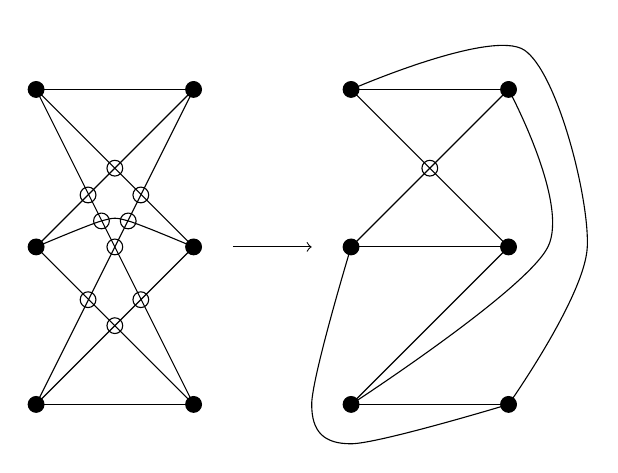
\begin{tikzpicture}
			\draw (0,0) -- (2,0);
			\draw (0,0) -- (2,2);
			\draw (0,0) -- (2,4);
			\draw (0,2) -- (2,0);
			\draw plot [smooth] coordinates {(0,2) (0.83,2.33) (1.17,2.33) (2,2)};
			\draw (0,2) -- (2,4);
			\draw (0,4) -- (2,0);
			\draw (0,4) -- (2,2);
			\draw (0,4) -- (2,4);
			\draw [fill=black] (0,0) circle (0.1);
			\draw [fill=black] (0,2) circle (0.1);
			\draw [fill=black] (0,4) circle (0.1);
			\draw [fill=black] (2,0) circle (0.1);
			\draw [fill=black] (2,2) circle (0.1);
			\draw [fill=black] (2,4) circle (0.1);
			\draw (1,1) circle (0.1);
			\draw (0.66,1.33) circle (0.1);
			\draw (1.33,1.33) circle (0.1);
			\draw (1,2) circle (0.1);
			\draw (0.83,2.33) circle (0.1);
			\draw (1.17,2.33) circle (0.1);
			\draw (0.66,2.66) circle (0.1);
			\draw (1.33,2.66) circle (0.1);
			\draw (1,3) circle (0.1);
			
			\onslide<2->{
				\draw [->] (2.5,2) -- (3.5,2);
				
				\draw (4,0) -- (6,0);
				\draw (4,0) -- (6,2);
				\draw plot [smooth] coordinates {(4,0) (6.5,2) (6,4)};
				\draw plot [smooth] coordinates {(4,2) (3.5,0) (4,-0.5) (6,0)};
				\draw (4,2) -- (6,2);
				\draw (4,2) -- (6,4);
				\draw plot [smooth] coordinates {(4,4) (6.2,4.5) (7,2) (6,0)};
				\draw (4,4) -- (6,2);
				\draw (4,4) -- (6,4);
				\draw [fill=black] (4,0) circle (0.1);
				\draw [fill=black] (4,2) circle (0.1);
				\draw [fill=black] (4,4) circle (0.1);
				\draw [fill=black] (6,0) circle (0.1);
				\draw [fill=black] (6,2) circle (0.1);
				\draw [fill=black] (6,4) circle (0.1);
				\draw (5,3) circle (0.1);
			}
		\end{tikzpicture}
	\end{figure}

	\onslide<2->{
		\begin{align*}
			kr(K_{3,3}) = 1
		\end{align*}
	}
\end{frame}

\begin{frame}[fragile]{Minimale Zeichnung}
	\begin{figure}
		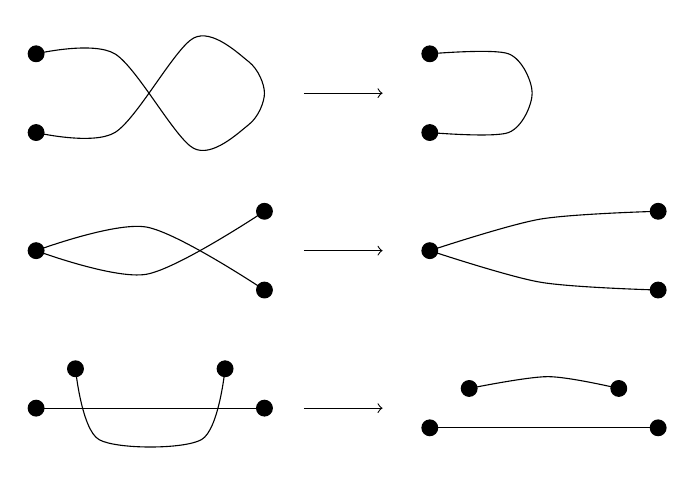
\begin{tikzpicture}
			\draw plot [smooth] coordinates {(0,0) (1,0) (2,1.2) (2.7,0.9) (2.9,0.5) (2.7,0.1) (2,-0.2) (1,1) (0,1)};
			\draw [fill=black] (0,0) circle (0.1);
			\draw [fill=black] (0,1) circle (0.1);
	
			\draw [->] (3.4,0.5) -- (4.4,0.5);
	
			\draw plot [smooth] coordinates {(5,0) (6,0) (6.3,0.5) (6,1) (5,1)};
			\draw [fill=black] (5,0) circle (0.1);
			\draw [fill=black] (5,1) circle (0.1);

			\onslide<2->{
				\draw plot [smooth] coordinates {(0,-1.5) (1.4,-1.8) (2.9,-1)};
				\draw plot [smooth] coordinates {(0,-1.5) (1.4,-1.2) (2.9,-2)};
				\draw [fill=black] (0,-1.5) circle (0.1);
				\draw [fill=black] (2.9,-2) circle (0.1);
				\draw [fill=black] (2.9,-1) circle (0.1);
	
				\draw [->] (3.4,-1.5) -- (4.4,-1.5);
				
				\draw plot [smooth] coordinates {(5,-1.5) (6.4,-1.9) (7.9,-2)};
				\draw plot [smooth] coordinates {(5,-1.5) (6.4,-1.1) (7.9,-1)};
				\draw [fill=black] (5,-1.5) circle (0.1);
				\draw [fill=black] (7.9,-2) circle (0.1);
				\draw [fill=black] (7.9,-1) circle (0.1);
			}
			
			\onslide<3->{
				\draw plot [smooth] coordinates {(0,-3.5) (2.9,-3.5)};
				\draw plot [smooth] coordinates {(0.5,-3) (0.8,-3.9) (2.1,-3.9) (2.4,-3)};
				\draw [fill=black] (0.5,-3) circle (0.1);
				\draw [fill=black] (2.4,-3) circle (0.1);
				\draw [fill=black] (0,-3.5) circle (0.1);
				\draw [fill=black] (2.9,-3.5) circle (0.1);
				
				\draw [->] (3.4,-3.5) -- (4.4,-3.5);
				
				\draw plot [smooth] coordinates {(5.5,-3.25) (6.5,-3.1) (7.4,-3.25)};
				\draw plot [smooth] coordinates {(5,-3.75) (7.9,-3.75)};
				\draw [fill=black] (5.5,-3.25) circle (0.1);
				\draw [fill=black] (7.4,-3.25) circle (0.1);
				\draw [fill=black] (5,-3.75) circle (0.1);
				\draw [fill=black] (7.9,-3.75) circle (0.1);
			}
		\end{tikzpicture}
	\end{figure}
\end{frame}

\begin{frame}{Erste Untere Schranke}
	\begin{framed}
		\begin{satz}
			\vspace{2.5mm}
			Sei \( G \) ein Graph mit \( n \) Knoten und \( m \) Kanten. Dann gilt
			\begin{align*}
				kr(G) \geq m - 3n + 6
			\end{align*}
		\end{satz}
	\end{framed}
	
	\textit{Beweis.}
\end{frame}

\begin{frame}{Erste Untere Schranke}
	\begin{figure}
		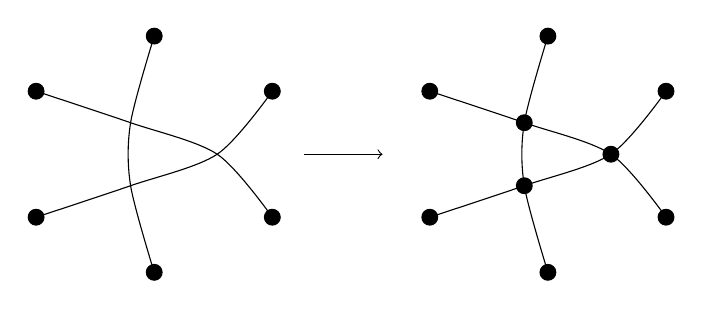
\begin{tikzpicture}
			\draw plot [smooth] coordinates {(0,0.7) (1.2,1.1) (2.3,1.5) (3,2.3)};
			\draw plot [smooth] coordinates {(0,2.3) (1.2,1.9) (2.3,1.5) (3,0.7)};
			\draw plot [smooth] coordinates {(1.5,0) (1.2,1.1) (1.2,1.9) (1.5,3)};
			\draw [fill=black] (0,0.7) circle (0.1);
			\draw [fill=black] (3,0.7) circle (0.1);
			\draw [fill=black] (0,2.3) circle (0.1);
			\draw [fill=black] (3,2.3) circle (0.1);
			\draw [fill=black] (1.5,0) circle (0.1);
			\draw [fill=black] (1.5,3) circle (0.1);
			
			\onslide<2->{
				\draw [->] (3.4,1.5) -- (4.4,1.5);
			
				\draw plot [smooth] coordinates {(5,0.7) (6.2,1.1) (7.3,1.5) (8,2.3)};
				\draw plot [smooth] coordinates {(5,2.3) (6.2,1.9) (7.3,1.5) (8,0.7)};
				\draw plot [smooth] coordinates {(6.5,0) (6.2,1.1) (6.2,1.9) (6.5,3)};
				\draw [fill=black] (5,0.7) circle (0.1);
				\draw [fill=black] (8,0.7) circle (0.1);
				\draw [fill=black] (5,2.3) circle (0.1);
				\draw [fill=black] (8,2.3) circle (0.1);
				\draw [fill=black] (6.5,0) circle (0.1);
				\draw [fill=black] (6.5,3) circle (0.1);
				\draw [fill=black] (7.3,1.5) circle (0.1);
				\draw [fill=black] (6.2,1.1) circle (0.1);
				\draw [fill=black] (6.2,1.9) circle (0.1);
			}
		\end{tikzpicture}
	\end{figure}

	Annahme: \( G \) mit \( n_G \) Knoten und \( m_G \) Kanten ist mit \( kr(G) \) Kreuzungen gezeichnet.
	
	\onslide<2->{
		Es wird \( H \) mit \( n_H = n_G + kr(G) \) Knoten, \( m_H = m_G + 2\,kr(G) \) Kanten und keinen Kreuzungen aus \( G \) erzeugt.
	}
\end{frame}

\begin{frame}{Erste Untere Schranke}
	\textbf{Eulersche Formel}
	
	Ein ebener Graph mit \( n \) Knoten und ohne Kreuzungen kann maximal \( 3n - 6 \) Kanten haben.
	
	\begin{align*}
		\onslide<2->{
			m_H	&\leq 3n_H - 6 \\
		}
		\onslide<3->{
			m_G + 2\,kr(G)	&\leq 3\,(n_G + kr(G)) - 6 \\
			m_G + 2\,kr(G)	&\leq 3n_G + 3\,kr(G) - 6 \\
		}
		\onslide<4->{
			m_G - 3n_G + 6	&\leq kr(G) \\
			kr(G)			&\geq m_G - 3n_G + 6
		}
		\only<4->{
			\pushQED{\qed} 
			\qedhere
			\popQED
		}
	\end{align*}
\end{frame}

\begin{frame}{Erste Untere Schranke}
	\begin{align*}
		kr(K_{3,3})	&\geq m_{K_{3,3}} - 3n_{K_{3,3}} + 6 \\
		kr(K_{3,3})	&\geq 9 - 3 \cdot 6 + 6 \\
		kr(K_{3,3})	&\geq -3 \\
		kr(K_{3,3})	&= 1 \\
		\\
		\onslide<2->{
			kr(K_6)	&\geq m_{K_6} - 3n_{K_6} + 6 \\
			kr(K_6)	&\geq 15 - 3 \cdot 6 + 6 \\
			kr(K_6)	&\geq 3
		}
	\end{align*}
\end{frame}

\begin{frame}{Kreuzungszahl von \( K_6 \)}
	\begin{figure}
		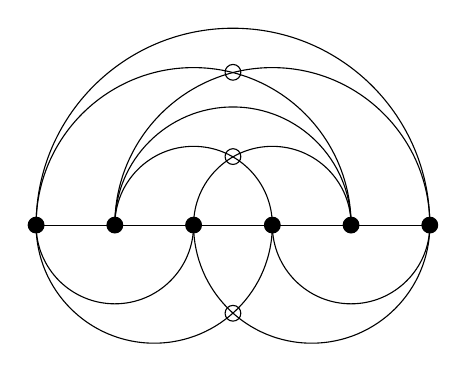
\begin{tikzpicture}
			\draw (0,0) -- (5,0);
			\draw (0,0) arc (180:360:1);
			\draw (0,0) arc (180:360:1.5);
			\draw (0,0) arc (180:0:2);
			\draw (0,0) arc (180:0:2.5);
			\draw (1,0) arc (180:0:1);
			\draw (1,0) arc (180:0:1.5);
			\draw (4,0) arc (0:180:1);
			\draw (5,0) arc (360:180:1);
			\draw (5,0) arc (360:180:1.5);
			\draw (5,0) arc (0:180:2);
			\draw [fill=black] (0,0) circle (0.1);
			\draw [fill=black] (1,0) circle (0.1);
			\draw [fill=black] (2,0) circle (0.1);
			\draw [fill=black] (3,0) circle (0.1);
			\draw [fill=black] (4,0) circle (0.1);
			\draw [fill=black] (5,0) circle (0.1);
			\draw (2.5,-1.12) circle (0.1);
			\draw (2.5,0.87) circle (0.1);
			\draw (2.5,1.94) circle (0.1);
		\end{tikzpicture}
	\end{figure}

	\begin{align*}
		kr(K_6) = 3
	\end{align*}
\end{frame}

\begin{frame}{Zweite Untere Schranke}
	\begin{framed}
		\begin{satz}
			\vspace{2.5mm}
			Sei \( G \) ein Graph mit \( n \) Knoten und \( m \) Kanten, wobei \( m \geq 4n \). Dann gilt
			\begin{align*}
				kr(G) > \frac{1}{64} \, \frac{m^3}{n^2}
			\end{align*}
		\end{satz}
	\end{framed}

	\textit{Beweis.}
\end{frame}

\begin{frame}{Zweite Untere Schranke}
	Es wird ein Untergraph \( G_p \) von \( G \) erzeugt, in dem jeder Knoten mit der Wahrscheinlichkeit \( p \) enthalten ist.
	
	\onslide<2->{
		Zufallsvariablen für \( G_p \):
		\begin{itemize}
			\item \textbf{Anzahl der Knoten} \( n_p \). \( E(n_p) = pn \)
			\item \textbf{Anzahl der Kanten} \( m_p \). \( E(m_p) = p^2m \)
			\item \textbf{Anzahl der Kreuzungen} \( X_p \). \( E(X_p) = p^4\,kr(G) \)
		\end{itemize}
	}%
	\onslide<3->{
		\begin{align*}
			m &\geq 4n \\
			p &= \frac{4n}{m} \implies p \leq 1 \\
		\end{align*}
	}
\end{frame}

\begin{frame}{Zweite Untere Schranke}
	\begin{align*}
		kr(G) - m + 3n	&> 0 \\
		\onslide<2->{
			E(X_p - m_p + 3n_p)		&> 0 \\
			p^4\,kr(G) - p^2m + 3pn	&> 0 \\
		}
		\onslide<3->{
			p^4\,kr(G)	&> p^2m - 3pn \\
			kr(G)		&> \frac{m}{p^2} - \frac{3n}{p^3} \\
			kr(G)		&> \frac{m^3}{16n^2} - \frac{3nm^3}{64n^3} \\
			kr(G)		&> \frac{4m^3}{64n^2} - \frac{3m^3}{64n^2} \\
			kr(G)		&> \frac{1}{64} \, \frac{m^3}{n^2}
		}
		\only<3->{
			\pushQED{\qed} 
			\qedhere
			\popQED
		}
	\end{align*}
\end{frame}